\documentclass[a4paper, 11pt, titlepage]{jsarticle}
\usepackage[dvipdfmx]{graphicx}
\usepackage{listings}
\usepackage{amsmath}
\usepackage{url}
\usepackage{here}


\title{知能情報実験III(データマイニング班)\\指紋認証を用いたCNNの手法についての模索}
\author{\textbf{185710A 金城海斗}\\
\textbf{185714C 石橋竜弥}\\
 \textbf{185745C 上間翔}\\
 \textbf{185752F 新垣裕二}\\
 \textbf{185763B 草薙幸菜}}
\date{提出日:2021年2月9日}
\begin{document}
\maketitle
\tableofcontents
\clearpage


\section{はじめに}
データマイニングとはデータの中に埋め込まれている有用な知識を発掘することである。別の言い方では、データマイニングは、より良い意思決定をするために履歴データをうまく使って一般的な規則性を発見しよとする研究分野である。今回私たちのグループ3では、機械学習の基本的な考え方を実装、体験を通して学んだ。そしてその応用として、既存に存在する指紋データを使った指紋認証のプログラムの分析から、畳み込みニューラルネットワークの手法についての模索、改善を行い、結果の精度向上を目指し、考察したことについて報告する。
\section{概要}
本グループでは機械学習の基本的な考えを学びそれを応用するために、指紋を畳み込みニューラルネットワークを用いて指紋の持ち主や左右どの指であるかを識別を行なった。
畳み込みニューラルネットワークとは、ある特徴を持つ画像をフィルタに畳み込んでいくことによってその画像の特徴を抽出する識別手法である。指紋の識別を対象にした理由としては、ラベルが明確であることと特徴が複雑であると考えたからである。
本実験の目的は、CNNのパラメータを変更し識別の精度を向上させ、得られた結果を考察し、CNNについて理解を深めることである。
具体的な識別の内容としてはある指紋が、「誰のものであるか」「左右十本のうちどの指であるか」の2種類の識別を行う。
実験結果としては、エポック数、バッチサイズ、活性化関数などを変更したが、どの場合についても識別率が99.8\%から大きく変わることはなかった。エポック数による精度の向上はやや見られたが、活性化関数が識別にどのような効果をもたらしているのかは読み取ることができなかった。
実験全体を通し、当初予定していた計画通りに進めることができた。しかし、バージョン管理やユニットテストについては、多くは行えなかったためそれらが今後な課題となる。
\subsection{Convolutional Neural Network:CNN}
Convolutional Neural Network (これよりCNNと呼ぶ)は畳み込みニューラルネットワークという意味であり、機械学習で画像の深層学習といえばCNNであるというほどよく使われている識別手法である。これは、ニューラルネットワークに畳み込みという操作を導入したものである。CNNについて、簡単な手順を記述する。まず手順1として、\textbf{画像から特徴を抽出}する。フィルタを使い、入力層データの中で位置を変えながらスキャンした部分のデータと、フィルター自身の持つデータとの差異を畳み込みの結果として畳み込みそうに書き込んだものを特徴量といい、入力層の全データをスキャンしてできた畳み込み結果の値の集まりを特徴マップという。複数のフィルタを用意することで、入力層のデータ特徴を捉えやすくしている。\textbf{図~\ref{cnn1}}は用意した複数フィルタのうち、一つが完全に入力層のデータの一部と同じであることを示す。

\begin{figure}[h]
  \centering
  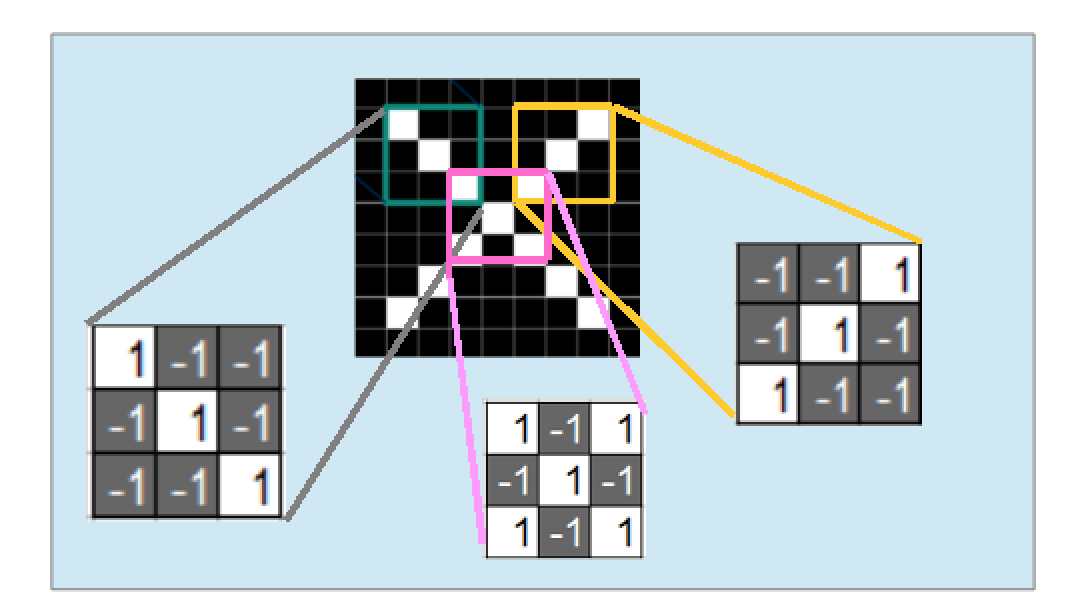
\includegraphics[scale=0.4]{cnn1.png}
  \caption{CNN解説手順1(参考サイト\cite{cnn}より引用)}
  \label{cnn1}
\end{figure}


手順2として、\textbf{画像を畳み込み}する。入力層のデータをフィルターのデータとピクセル毎に比較することで、畳み込み層にその類似度(特徴量)を書き込む。\textbf{図~\ref{cnn2}}はフィルタを利用して特徴量を抽出し、特徴マップを作成した例である。

\begin{figure}[h]
  \centering
  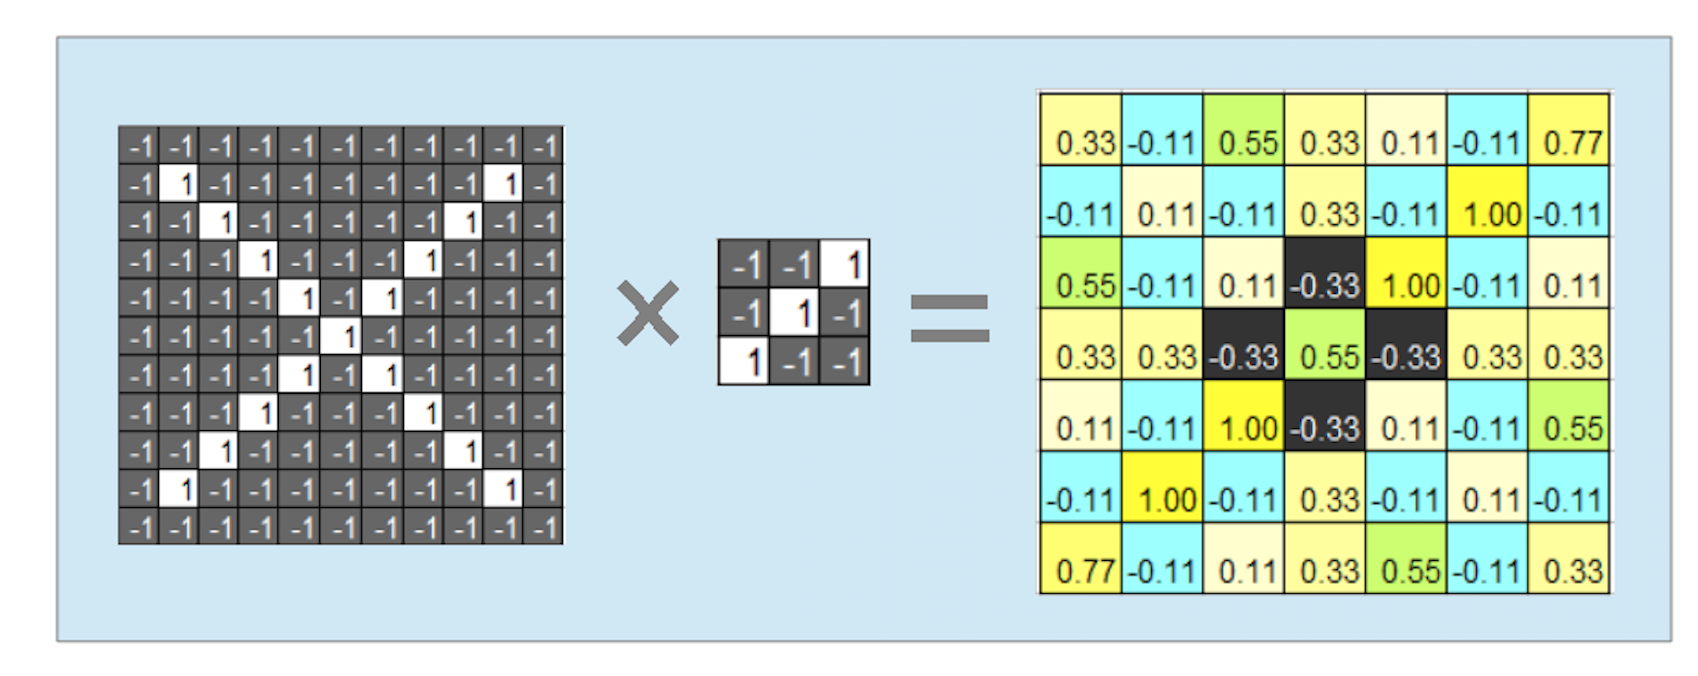
\includegraphics[scale=0.3]{cnn2.png}
  \caption{CNN解説手順2(参考サイト\cite{cnn}より引用)}
  \label{cnn2}
\end{figure}

手順3として、\textbf{画像をプーリング}する。畳み込みの層の情報はプーリング層で集約する。出力に関しては、プーリング層のユニット全てと全結合し、計算結果を利用して、フィルタ、重み、バイアスを更新していく。(\textbf{図~\ref{cnn3}})

\begin{figure}[h]
  \centering
  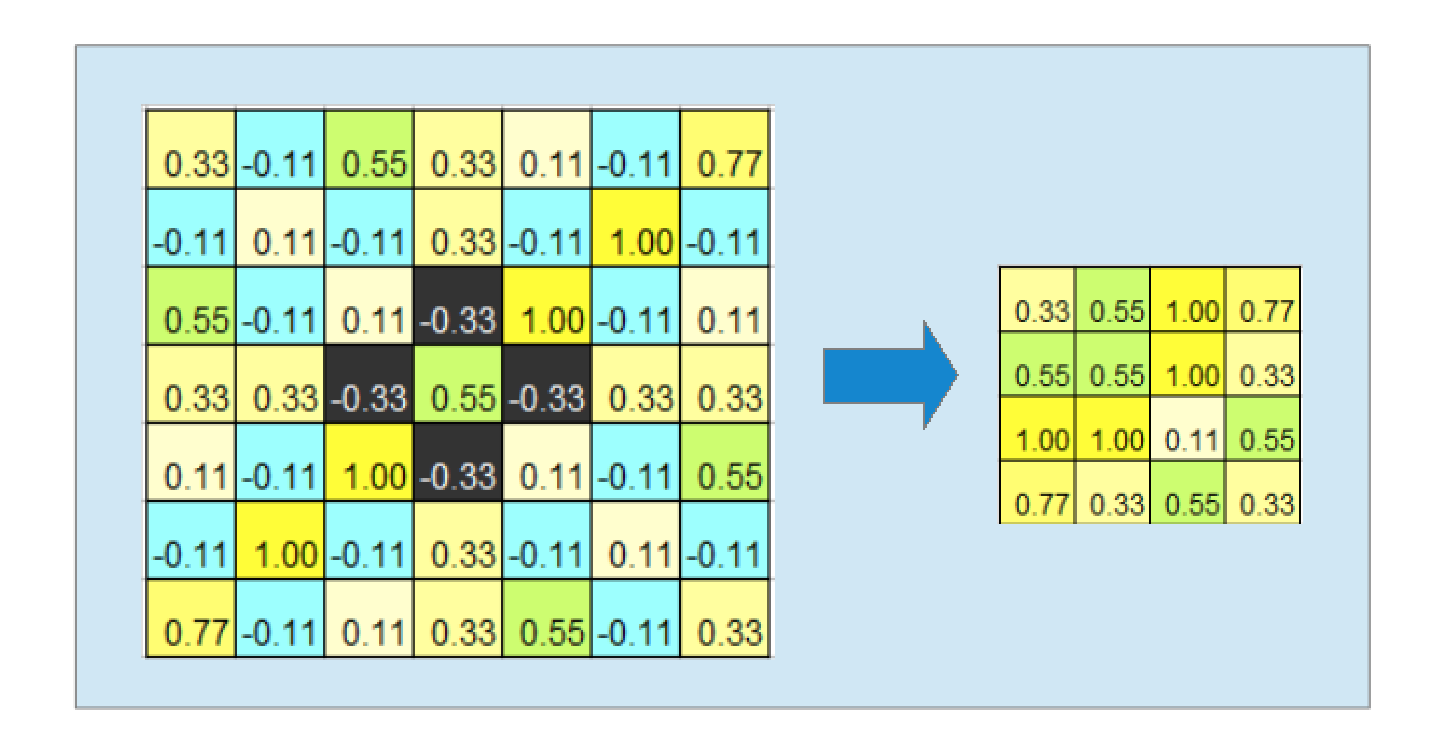
\includegraphics[scale=0.3]{cnn3.png}
  \caption{CNN解説手順3(参考サイト\cite{cnn}より引用)}
  \label{cnn3}
\end{figure}


\subsection{テーマ指紋認証とは}
本グループでは、授業の中でデータマイニングについて学び、それらの応用実験として、画像認識について分析しようと考えた。そして、データマイニングを行う識別手としてCNNに目をつけ、データの分類ラベルがはっきりしており、複雑である指紋認証の分析、精度改善を行うこととなった。CNNは畳み込み処理を利用したニューラルネットワークであり、どのくらい畳み込み処理を行うのか、どのくらいニューラルネットワークを深くするのかは定義されていない。


\section{実験方法}


\subsection{実験目的}
本実験では大きく3つを目的にあげる。1つ目に、指紋データセットを用いて指紋認証をCNNというアルゴリズムを使って行っているが、CNNというデータマイニングの画像認識の手法の一つを理解し、実行することを目的とする。二つ目に、CNNのパラメータ調整をいくつか行っていくことで、指紋認証の識別率の改善、結果向上も目的にある。さらに、三つ目として、各々パラメータ調整によってどのような違いがうまれるのか等を可視化を通しながら考察していくことを目的とする。


\subsection{データセット構築}
Kaggleより、指紋のデータセット\cite{cnn}を利用している。

\subsection{モデル選定}
アルゴリズムは序章で述べたとおり、CNNを利用しており、SubjectID\&Finger\_CNNRecognizer
\cite{algorithm}のコードを参考にしている。

本アルゴリズムの運用において、指紋認証の正答率が十分に高い点、可読性に優れており改善手法を模索しやすい点に特に優れているため使用することにした。

\subsection{パラメータ調整}
CNNのパラメータ調整では、epoch数・画像データ数・batchsizeや活性化関数であるLeakyReLUを変更していった。


%\newpage
\section{実験結果}

実験結果を以下の表\ref{change:epoch}から表\ref{change:activation}に示す。今回は、指紋の持ち主の識別と、左右のどの指かの識別の2種類の識別を行った。そのため、指紋の持ち主の識別率をsubjectID accracy、左右のどの指かの識別率をfingerNum accracyで表している。
%事実として得られた結果を示そう。
%なお、以下の点に留意すること。
%ここの条件(batch_sizeとかmodelの中身とか)の補足をお願いします。
%epoch10の値の共通項がコピペ事故起こしてそうですが大丈夫ですか?

\begin{table}[htb]
\begin{center}
\caption{エポック数を1から30までの値に変更}
  \begin{tabular}{|l|c|c|}
    \hline
    epoch & subjectID accracy & fingerNum accracy \\ \hline
    1 & 01.533 \% & 63.016 \%  \\ \hline
    3 & 61.283 \% & 89.483 \% \\ \hline
    5 & 96.350 \% & 98.150 \%  \\ \hline
    10 & 99.716 \% & 99.716 \%  \\ \hline
    20 & 99.733 \% & 99.883 \%  \\ \hline
    30 & 99.733 \% & 99.900 \% \\ \hline
  \end{tabular}
  \label{change:epoch}
 \end{center}
\end{table}

%アンダーバーは関数記号?エラーの元。ただの記号にするためのバックスラッシュが必要
\begin{table}[htb]
\begin{center}
\caption{epochを20に固定し、batch\_sizeを変更}
  \begin{tabular}{|l|c|c|}
    \hline
    batch\_size & subjectID accuracy & fingerNum accuracy  \\ \hline
    32 & 99.733 \% & 99.900 \% \\ \hline
    64 & 99.733 \% & 99.883 \% \\ \hline
    128 & 99.716 \% & 99.883 \% \\ \hline
  \end{tabular}
    \label{change:batch}
\end{center}
\end{table}

%ここの条件(batch_sizeとかepochとか)の補足をお願いします。
\begin{table}[htb]
\begin{center}
\caption{活性化関数をLeakyReLU、sigmoid、tanhに変更}
  \begin{tabular}{|l|c|c|}
    \hline
    活性化関数 & subjectID accracy & fingerNum accracy \\ \hline
    LeakyReLU (alpha=$-0.5$) & 99.433 \% & 99.883 \% \\ \hline
    LeakyReLU (alpha=0.3) & 99.716 \% & 99.733 \% \\ \hline
    LeakyReLU (alpha=0.5) & 99.699 \% & 99.633 \% \\ \hline
    sigmoid & 99.733 \% & 99.866 \% \\ \hline
    tanh & 99.733 \% & 99.883 \% \\ \hline
  \end{tabular}
    \label{change:activation}
 \end{center}
\end{table}

\section{考察}
初めに、元のサンプルコードの条件はエポック数20のバッチサイズ64、活性化関数は中間層でReLU関数を用いて、出力層に対してsoftmax関数を用いている。結論から言うと、どの条件下においても大きな変化は見られなかった。精度を向上させることができた条件は、エポック数を20から30に増やすこと、バッチサイズを64から32に変更することの2つであった。また、両者とも精度が上がったのは fingerNum accracyのみであった。この原因と、その他の条件において精度が上昇しなかった原因について考える。

初めに、fingerNum accracyのみ精度が向上したことについて考える。エポック数とは学習する世代のことであり、これを多くしていくことで細かい識別が可能になる。今回の結果から考えると、fingerNum accracyの方が識別により細かい特徴を必要とすると考える。

次に、活性化関数を変更した場合について考える。今回は画像の識別であるため、活性化関数も多くの値を表現できるものが良いと考えた。0と1だけで識別するのと、1から100までを用いて識別するのは後者の方がより細かいものを表現できるはずである。実際、元のサンプルコードは負の値は0にし、正の値はそのまま使用するReLU関数を用いていた。そこで、負の値も一定の割合で使用するLeakyReLU関数を用いたが結果は精度がやや落ちる程度だった。また、sigmoid関数とtanh関数も用いた。これらは入力された値を、0から1、-1から1の実数にする関数である。これまでの考えだと精度は下がると予測したが、LeakyReLU関数を用いた結果とあまり大差はなかった。これらのことを見ると活性化関数に精度との相関が見られない。活性化関数の他に精度をあげている要因があると考えられる。今回の実験では最適化関数について変更を行っていため、最適化関数に原因があるのではないかと考える。

以上より、エポック数による精度の向上はやや見られたが、活性化関数が識別にどのような効果をもたらしているのかは読み取ることができなかった。

\newpage%ここだけ改行入れてます。
\section{意図していた実験計画との違い}
%グループワークとして2ヶ月程度の時間が用意されていた。
%ガントチャート\ref{ganttchart}等、何かしら工夫して全体の計画を述べよう。
%これらの期間をどのように使おうとし、実際どうだったのかについて自己評価(振り返り)してみよう。
%大きなズレがある場合それは何故起きたのか、どうやればそのギャップを縮められそうか検討してみよう。

%https://ctan.org/pkg/pgfgantt
当初予定していた実験計画は以下の通りとなる。
下記の予定は11月17日に作成されたものである。後々詳しく決められた締め切り予定には(追加内容:)として記述する。%ラベルじゃ無いけど。

%超絶めんどくさくなった。
\begin{table}[H]
	\begin{tabular}{|l|l|l|}
		\hline
		講義時間(日次) & 実験計画 & 実際に行った内容	\\ \hline \hline
		6週目(11/17)
		 &\begin{tabular}{l}
		 	テーマ決め\\
			データセット探し\\
			など
		\end{tabular}
		 & \begin{tabular}{l}
		 	テーマ決定(画像認証/fingerprint)\\
			データセット探し\\
			画像認証に対しての学習
		\end{tabular}	\\ \hline
		7週目(11/24)
		 &\begin{tabular}{l}
		 	特徴ベクトルの抽出や\\
			コード探して理解する
		\end{tabular}
		 &\begin{tabular}{l}
		 	指紋の特徴量の分析\\
			CNNの画像認証コードの検索
		\end{tabular}	\\ \hline
		8週目(12/1)
		 &\begin{tabular}{l}
		 画像認識をコードに落とし込む\\
		 \end{tabular}
		 &\begin{tabular}{l}
		 	参考するCNNコードの決定\\
			コードの内容の分析・実行
		\end{tabular}		\\ \hline
		9週目(12/8) 
		 &\begin{tabular}{l}
		 	実験開始\\
			出来上がったコードを動かす
		\end{tabular}
		 &\begin{tabular}{l}
		 	コードの内容の分析\\
			実行2nd
		\end{tabular}	\\ \hline
		10週目(12/15)
		 &\begin{tabular}{l}
		 コードや特徴ベクトルの調整\\
		 \end{tabular}
		 &\begin{tabular}{l}
		 	コードの内容の分析3rd\\
			amaneによる実行開始\\
			実験目的の草案作成
		\end{tabular}	\\ \hline
		11週目(12/22)
		 &\begin{tabular}{l}
		 未決定\\
		 \end{tabular}
		 &\begin{tabular}{l}
		 	コードの内容の分析4th・実行2nd\\
			amaneで画像データ作成は難しいと判断\\
			来年に向けての引継ぎ
		\end{tabular}	\\ \hline
		12週目(1/5)
		 &\begin{tabular}{l}
		 	未決定
		\end{tabular}
		 &\begin{tabular}{l}
		 	コードの内容の分析5th\\
			epoch数を変えた大規模実験\\
			Python/Keras環境の統一
		\end{tabular}	\\ \hline
		13週目(1/12)
		 &\begin{tabular}{l}
		 	改善実験
		\end{tabular}
		 & \begin{tabular}{l}
		 	コードの内容の分析6th\\
			batch\_sizeやLeakyReLUを変更した実験
		\end{tabular}	\\ \hline
		14週目(1/19)
		 &\begin{tabular}{l}
		 	未決定
		\end{tabular}
		 &\begin{tabular}{l}
		 	レポートの作成\\
			amaneによる実験 
		\end{tabular}	\\ \hline
		15週目(1/26)
		 &\begin{tabular}{l}
		 	レポート・プレゼン資料作成\\
			(追加内容:レポート初期版の提出日)
		\end{tabular}
		 &\begin{tabular}{l}
		 	レポート・プレゼン資料作成\\
			レポート初期版の作成
		\end{tabular}	\\ \hline
		(1/26) &  
		&\begin{tabular}{l}
			レポート・プレゼン資料作成
		\end{tabular}	\\ \hline
		期末日(2/2) 
		&\begin{tabular}{l}
			最終発表
		\end{tabular} 
		&\begin{tabular}{l}
		最終発表
		\end{tabular}	\\ \hline
		(2/16) 
		&\begin{tabular}{l}
			(追加内容:Github公開)
		\end{tabular}
		&\begin{tabular}{l}
			公開済み
		\end{tabular}	\\ \hline
	\end{tabular}
\end{table}

実験計画を作成した段階では後半の進捗の進み具合の判断が困難だったため、前半の予定と締め切りに合わせた大まかな目標を設定し、他は未定とした。未定の欄を除いて概ね実験計画と実際の進捗に大きな乖離はなく、順調に進んだと判断できる。


\section{まとめ}
本実験のデータマイニング班の達成目標を大まかにまとめると、バージョン管理やユニットテストを用いながら機械学習やデータセットの可視化や構築をできるようになるというものである。

今回、本グループはサンプルコードを改良し結果を向上させる形で実験に取り組んだ。そのため、データセットについては既に構築されており、コードについてもjupyterで編集する形であったため、バージョン管理やユニットテストについては多くは行わなかった。しかし、開発に時間を割かなかった分、本実験で使用したCNNの畳み込みやプーリング、活性化関数といった構造を理解することができた。そこからCNNによる識別率の向上に寄与する要因を考察し手を加え、さらに得られた結果から自分たちが修正したものがどのような影響を及ぼしたのかについても考察することができた。また作業においても役割を分担し、計画通りに進めることができた。

\section{振り返り}
今後の課題としてはまとめで述べたように、バージョン管理、ユニットテスト、自力でのコーディングが行えなかったので、自分たちでコーディングできるようになり、そのコードに対しバージョン管理、ユニットテストを行えるようになることが考えられる。大まかにスケジュールを組むならば、用いるライブラリの打ち合わせ、用いる学習器の決定、その後コーディングに入るとスムーズにいくと考えられる。


\begin{thebibliography}{n}
  \bibitem{cnn}
「畳み込みニューラルネットワークとは?手順も丁寧に解説」, \\
  \textless \url{https://udemy.benesse.co.jp/data-science/ai/convolution-neural-network.html}\textgreater 2021/02/09.
  
  \bibitem{dataset}ruizgara「Sokoto Coventry Fingerprint Dataset (SOCOFing)」\\
  \textless \url{https://www.kaggle.com/ruizgara/socofing}\textgreater 2021/02/09.
  
  \bibitem{algorithm}Brian Zhang「SubjectID\&Finger\_CNNRecognizer」, \\
  \textless \url{https://www.kaggle.com/brianzz/subjectid-finger-cnnrecognizer}\textgreater 2021/02/09.
  
\end{thebibliography}

\end{document}
